\chapter{Background}
\label{chp:background}

In this chapter, some of the basic technical background to buffer overflows is explained.
\Cref{sec:process-memory} explains the basic memory layout of a process running on the Linux kernel.
\Cref{sec:stack-setup-and-usage} focuses on how the stack is used during program execution.
\Cref{sec:stack-buffer-overflows} finally presents what a stack buffer overflow is, how it can be exploited and why it is so dangerous.

\section{A process's memory}
\label{sec:process-memory}

When a program is executed, it has to be loaded into the computer's main memory before the kernel can hand the control flow to the newly-created process.
During that process, several sections of the \gls{elf} binary%
	\footnote{See e.g. the \href{https://en.wikipedia.org/wiki/Executable_and_Linkable_Format}{wikipedia.org} entry for further information on \gls{elf}}
are put straight into memory.
For example, the \texttt{.text} section containing the actual binary instructions for the program or the \texttt{.data} and \texttt{.bss} sections holding initialized and uninitialized global variables, respectively, are allocated at the lowest memory address of the process's virtual memory space.
The size of those sections is already known on program initialization which is why they can be allocated without the need of spare memory to grow those memory regions.

\begin{figure}[htb]
	\centering
	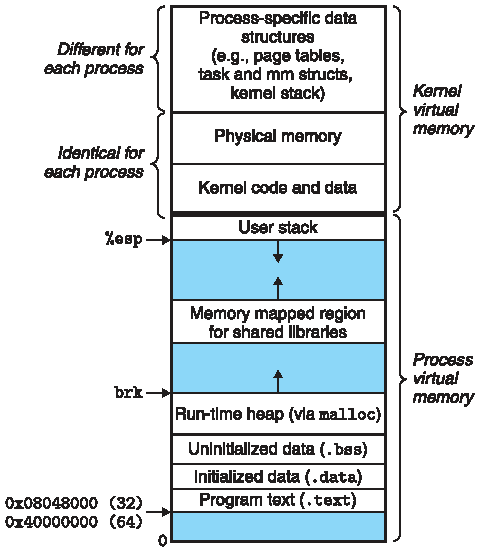
\includegraphics[width=0.5\textwidth]{figures/memory-layout}
	\caption{The memory layout of a Linux process \cite[804]{Bryant2011}}
	\label{fig:memory-layout}
\end{figure}

As \cref{fig:memory-layout} shows, above those memory regions the dynamically growing and shrinking memory regions like the heap, the mapped memory and the stack are located.
Those regions have in common that depending on the program's execution flow, their size changes.
Thus, they need to have free memory around them in order to be able to dynamically grow (marked in blue in \cref{fig:memory-layout}).

The heap contains data which has to be allocated dynamically because the necessary amount of memory is not fixed and has to be determined during runtime.
This includes for example arrays or buffers like the \texttt{input} buffer in \cref{lst:memory-layout}.
As the user input cannot be determined before running the program, the buffer has to be allocated dynamically which happens with a call to \texttt{malloc} in line 11 of the listing.
The contents of the buffer are then stored on the heap.

The stack on the other hand contains data with fixed size.
In the example of \cref{lst:memory-layout}, sizes of variables like \texttt{int max\_len} or \texttt{char *input} are known at compile-time.
Thus, they can be stored on the stack by increasing the stack by a fixed size when program flow enters the corresponding function.
It has to be noted here that even though the contents of the \texttt{input} buffer are stored in the heap, the pointer to those contents is stored on the stack.

The mapped memory is a region where files from the computers file system are mapped to directly address those files' contents just like other any other memory contents like variables or program instructions.
Such files can be any files accessible by the running program.
The main usage for this feature is to map libraries into memory, for example \gls{glibc} or custom created libraries.

\lstinputlisting[language=C,float=ht,caption={C program containing stack variables as well as heap variables},label={lst:memory-layout}]{code/memory-layout.c}

\section{Stack setup and usage}
\label{sec:stack-setup-and-usage}

As shown in \cref{sec:process-memory}, the stack can contain program data with a size already known at compile time.
When a function is entered, the stack size is increased by the accumulative size of the function's variables by decrementing the stack pointer by this size.
The stack pointer is stored in the processor register \texttt{esp} (\texttt{x86}/\texttt{i386} architecture) or \texttt{rsp} (\texttt{x86\_64}/\texttt{amd64} architecture) and points to the top of the stack.
On leaving the function, the stack size is decreased by the same amount of memory by incrementing the stack pointer.
This implies that variables declared in a function can only be safely accessed as long as the function is active.
``Active'' here means that either control flow is currently inside this function or inside another function called by this function, maybe even recursively.
Otherwise, the memory where those variables reside was already freed by decreasing the stack size and any access to such variables yields nondeterministic behavior.

When a function is called, not only its variables are stored on the stack but also the \gls{rip}.
The \gls{rip} points to the next instruction in the calling function which should be executed after the called function returns.
This is exactly what the \texttt{call} and \texttt{ret} assembly instructions do.
\texttt{call} pushes the address of the next instruction onto the stack and then enters the called function.
In the called function, \texttt{ret} at the end of the function pops the saved address from the stack and continues execution at this address.

Thus, the stack not only contains data but also important control flow information.

\section{Stack Buffer Overflows}
\label{sec:stack-buffer-overflows}

This mixture of data and control flow information is exactly where problems arise.

Under the assumption that a function exists somewhere in a program as shown in \cref{lst:vulnerable-function}, the stack layout of such a function may look as shown in \cref{fig:stack-layout-without-data}.
After the \gls{rip}, the compiler positions the \gls{sfp} (a pointer to the start of the previous stack frame) and the local variables in the order they were declared%
	\footnote{
		The layout as shown in \cref{fig:stack-layout} should just be seen as an example, as it can differ depending on compiler behavior or processor architecture (here: 32 bit architecture with stack alignment on 4 bytes, function arguments passed on the stack).
	}%
.

\begin{lstlisting}[language=C,float=ht,caption={C function with buffer overflow vulnerability}, label={lst:vulnerable-function}]
void copy(char *bar) {
char c[12];
strcpy(c, bar);
}
\end{lstlisting}

A stack buffer overflow vulnerability here lies in the call to \texttt{strcpy} in line 6.
This function copies a string from the memory location where \texttt{bar} points to to the memory location where \texttt{c} points to.
However, it copies data until it encounters a \texttt{0x00} byte which marks the end of the string, regardless of whether the destination can take all the copied data.

If the string to copy is strictly less than 12 bytes, no problem occurs as the buffer can hold the string (11 bytes at maximum) and the string terminating \texttt{0x00} byte as shown in \cref{fig:stack-layout-no-overflow}.

If the string to copy is 12 bytes or more, a buffer overflow occurs as shown in \cref{fig:stack-layout-overflow}.
This means that the \texttt{strcpy} function copies 12 bytes or more of data to the buffer \texttt{c} even though it cannot hold more than 12 bytes.
Including the terminating \texttt{0x00} byte, this string copy operation thus overwrites data residing on the stack after the destination buffer.

\begin{figure}[htb]
	\centering
	\begin{subfigure}[t]{0.3\textwidth}
		\centering
		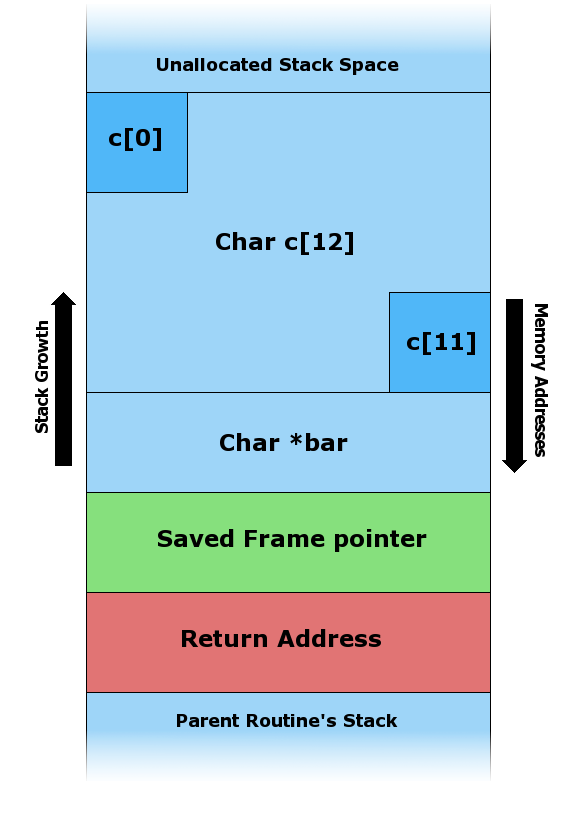
\includegraphics[height=0.25\textheight]{figures/Stack_Overflow_2}
		\caption{Stack layout with control flow information and local data \cite{Lynn2007}}
		\label{fig:stack-layout-without-data}
	\end{subfigure}
	\hfill
	\begin{subfigure}[t]{0.3\textwidth}
		\centering
		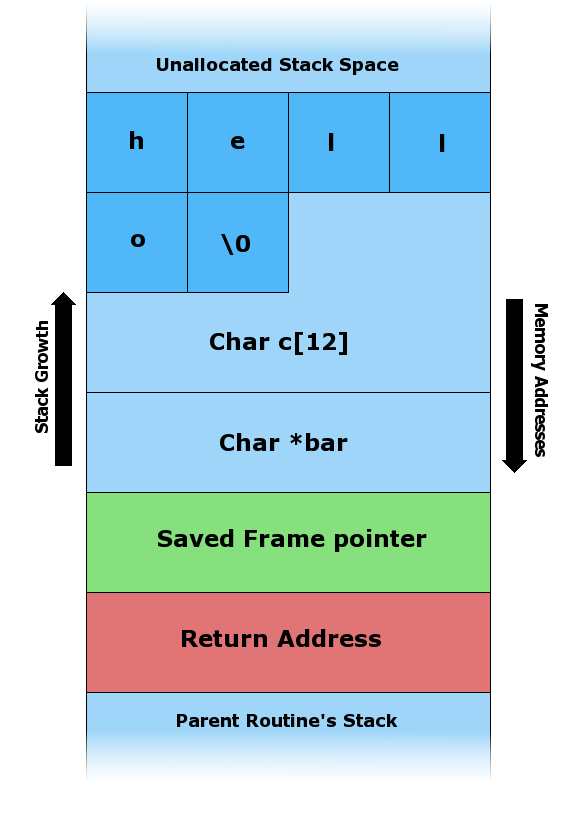
\includegraphics[height=0.25\textheight]{figures/Stack_Overflow_3}
		\caption{Stack contents after copying data to the \texttt{char} array without overflowing it \cite{Lynn2007a}}
		\label{fig:stack-layout-no-overflow}
	\end{subfigure}
	\hfill
	\begin{subfigure}[t]{0.3\textwidth}
		\centering
		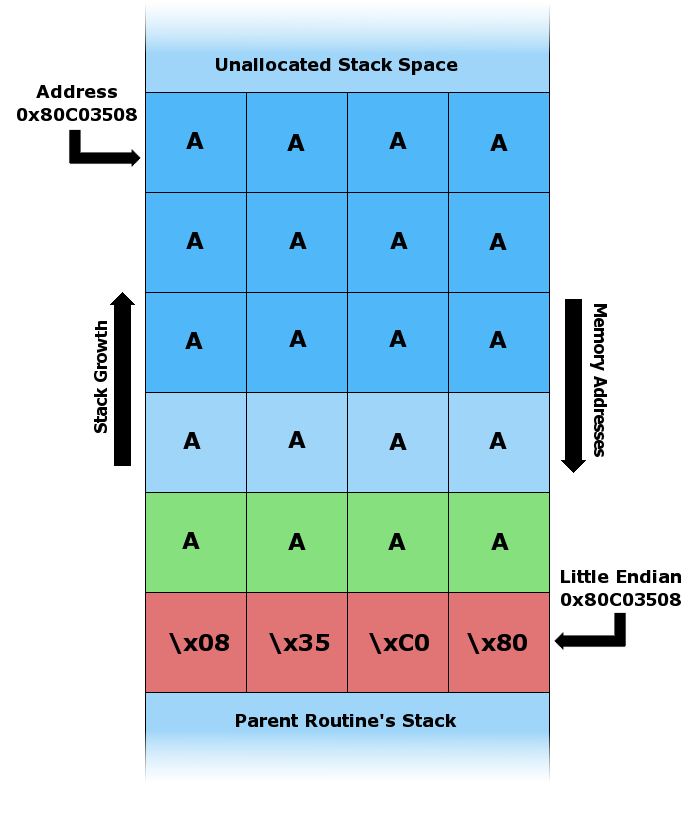
\includegraphics[height=0.25\textheight]{figures/Stack_Overflow_4}
		\caption{Stack contents after copying data to the \texttt{char} array and overflowing it \cite{Lynn2007b}}
		\label{fig:stack-layout-overflow}
	\end{subfigure}
	\caption{Stack layout of a function with two local variables: a 12 byte buffer (\texttt{char c[12]}) and a pointer (\texttt{char *bar})}
	\label{fig:stack-layout}
\end{figure}

If an attacker can control the data which is copied onto the stack, they can carefully craft an input string so that they can overwrite the \gls{rip} with attacker-controlled data and thus control where the program tries to continue execution after it returns from the current function.
A stack buffer overflow always occurs if a buffer just like \texttt{c} in \cref{lst:vulnerable-function} is filled with more data than it can hold.
This does not necessarily mean that the \gls{rip} is overwritten by a stack buffer overflow, but in most cases this is the goal of an attacker in order to divert control flow in the program's execution.

How an attacker can divert control flow and what implications come with this possibility is explained in \cref{chp:attack-vectors}.

